\documentclass[12pt,a4paper]{report}

\usepackage[margin=1in]{geometry}
\usepackage{amsmath}
\usepackage{amssymb}
\usepackage{graphicx}
\usepackage{hyperref}
\usepackage{booktabs}
\usepackage{setspace}
\usepackage{algorithm}
\usepackage{algpseudocode}
\usepackage{tikz}
\usetikzlibrary{arrows.meta,positioning,shapes.geometric,fit,calc}

\hypersetup{
    hidelinks
}

\newcommand{\chapterdesc}[1]{%
    \vspace{-0.6\baselineskip}
    \noindent\hspace*{1.5cm}\parbox{\dimexpr\textwidth-1.5cm\relax}{\textit{#1}}
    \par\vspace{0.3\baselineskip}
}

\begin{document}

\onehalfspacing

% ----------------------------
% Title page
% ----------------------------
\begin{titlepage}
    \centering
    
\includegraphics[height=2.6cm]{bk.png}\par
    \vspace{0.6cm}
    {\large VIETNAM NATIONAL UNIVERSITY\par}
    {\large UNIVERSITY OF TECHNOLOGY\par}
    {\large FACULTY OF COMPUTER SCIENCE AND ENGINEERING\par}
    \vspace{1.5cm}
    {\large\bfseries - FINAL PROJECT REPORT -\par}
    \vspace{1.0cm}
    {\Large\bfseries Book Recommendation System:\\Design, Machine Learning Pipeline, and Evaluation\par}
    \vspace{1.5cm}
    \begin{flushleft}
        \begin{tabular}{@{}l c l@{}}
            \textbf{Council}    & : & Computer Science \\
            \textbf{University} & : & Ho Chi Minh University of Technology \\
            \textbf{Faculty}    & : & Computer Science and Engineering \\
            \textbf{Instructor} & : & Prof. Quản Thành Thơ \\
            \textbf{Author}     & : & Đặng Thế Đông A (2570791) \\
            \textbf{Email}      & : & a.dangthedong@hcmut.edu.vn \\
            \textbf{Phone}      & : & 0902971858
        \end{tabular}
    \end{flushleft}
    \vspace{0.8cm}
    \begin{flushleft}
        \textbf{Project Links}
        \begin{itemize}
            \item \textbf{Link 1 (Shared Drive):} \url{https://drive.google.com/drive/folders/<shared-drive-id>}\\
                  \textit{Set permission to ``Anyone with the link -- Viewer'' and include: dataset, source code, and reproduction manuals.}
            \item \textbf{Link 2 (Demo Video):} \url{https://www.youtube.com/watch?v=<demo-video-id>}
        \end{itemize}
    \end{flushleft}
    \vfill
    {\large Ho Chi Minh City, May 2026\par}
\end{titlepage}

\clearpage
\pagenumbering{roman}

\chapter*{Declaration of Authenticity}
I declare that this report is my own work, conducted under the supervision of my instructor. The results and discussions presented in this report are original to this project context and have not been published previously in this form.

All materials, methods, and references adopted from prior works are properly cited in the References section. Any use of external ideas, datasets, and technical foundations is acknowledged in accordance with academic integrity requirements.

\clearpage
\chapter*{Acknowledgements}
I would like to express my sincere gratitude to my instructor and the members of the research group for their guidance, support, and valuable feedback throughout this project.

I also thank my family and friends for their continuous encouragement during the implementation and writing process of this report.

\clearpage
\chapter*{Abstract}
This report documents a full-stack book recommendation system that combines a React web frontend, a FastAPI backend, and a collaborative filtering model based on matrix factorization (implemented via stochastic gradient descent with latent factors, commonly referred to as SVD-style factorization) \cite{react,fastapi,matrix_factorization}. The system serves three stakeholder roles---end users, administrators, and data scientists---and is trained on the public Book-Crossing dataset \cite{bookcrossing}.

After preprocessing explicit ratings and training with 80 latent factors, the model achieves a test RMSE of \textbf{0.857} on held-out ratings, with binary classification metrics (threshold 3.5 stars) of \textbf{77.1\%} accuracy, \textbf{78.3\%} precision, \textbf{96.8\%} recall, and \textbf{86.6\%} F1-score. The report covers stakeholder benefits, algorithm theory, system architecture, data preprocessing, the AI training and deployment pipeline, and evaluation methodology.

\tableofcontents
\listoffigures
\listoftables
\clearpage

\pagenumbering{arabic}

\chapter{Introduction}
\chapterdesc{This chapter introduces the book recommendation problem, states the project objectives, defines scope and limitations, and outlines the structure of the remainder of this report.}

Personalized book recommendation helps readers discover relevant titles in large catalogs where manual browsing is inefficient. This project implements a production-style web application that ingests the Book-Crossing dataset, exposes REST APIs for catalog and user interactions, and deploys a trained collaborative filtering model to rank books for authenticated users.

\section{Objectives}
The project goals are:
\begin{itemize}
    \item Build a role-based web application (user, admin, data scientist).
    \item Train and evaluate an SVD-style matrix factorization model on real rating data.
    \item Persist model artifacts and serve personalized recommendations via API.
    \item Provide dashboards for catalog management, analytics, and model experimentation.
\end{itemize}

\section{Scope and Limitations}
The system uses the Book-Crossing CSV dumps for seeding and offline training. Inference relies on an \emph{item-centric} saved model (book biases and factors) with online estimation of user profiles from a small number of in-app ratings. When SVD recommendations are unavailable (for example, no user ratings), the API falls back to seeded recommendation rows when available, then to preference/popularity ranking. Analytics KPIs on the data scientist dashboard include seeded demonstration data for engagement trends.

\section{Report Structure}
The remainder of this report is organized as follows:
\begin{itemize}
    \item Chapter 2 identifies stakeholders and the benefits they derive from the system.
    \item Chapter 3 presents the theoretical background of recommendation algorithms used in this project.
    \item Chapter 4 describes the system design, including backend, frontend, and deployment flow.
    \item Chapter 5 documents the dataset and preprocessing steps.
    \item Chapter 6 details the AI pipeline for training and deployment.
    \item Chapter 7 reports evaluation results with quantitative metrics.
    \item Chapter 8 summarizes the user interface and concludes with future work directions.
\end{itemize}

\chapter{Stakeholder Analysis}
\chapterdesc{This chapter identifies the stakeholders involved in the project and explains the potential benefits each group can derive from the book recommendation system.}

\section{Stakeholder Identification}

Table~\ref{tab:stakeholders} summarizes the primary stakeholders, their roles in the system, and the interfaces they use.

\begin{table}[htbp]
\centering
\caption{Project stakeholders and system touchpoints}
\label{tab:stakeholders}
\begingroup
\renewcommand{\arraystretch}{1.25}
\setlength{\tabcolsep}{8pt}
\begin{tabular}{@{}p{3.2cm}p{4.2cm}p{6.6cm}@{}}
\toprule
\textbf{Stakeholder} & \textbf{Role} & \textbf{Touchpoints} \\
\midrule
End users (readers) &
Browse, search, rate books; manage reading list; receive recommendations &
Home (\texttt{/}), Search, Book Detail, Profile \\
Administrators &
Manage book catalog; view top-rated analytics &
Admin dashboard (\texttt{/admin}), \texttt{/api/v1/admin/*} \\
Data scientists &
Train/tune models; monitor metrics and experiments &
Data Scientist dashboard (\texttt{/data-scientist}), \texttt{/api/v1/ml/*} \\
Developers / maintainers &
Implement APIs, database, ML pipeline &
\texttt{backend/app/}, \texttt{Bookrecommendationsystemui/} \\
\bottomrule
\end{tabular}
\endgroup
\end{table}

\section{Benefits by Stakeholder}

\textbf{End users} benefit from personalized recommendations displayed on the home page, including a human-readable \texttt{reason} and a \texttt{predicted\_rating} score. Rating books improves future recommendations through online user profile estimation. Search and filters reduce discovery time; the reading list tracks planned, reading, and completed books.

\textbf{Administrators} maintain catalog quality via create/update/delete book operations and can monitor top-rated titles aggregated from the dataset. This supports content curation for a library or retail scenario.

\textbf{Data scientists} gain a reproducible training workflow: configurable hyperparameters, optional grid search over tuning spaces, persisted experiment history (\texttt{ModelExperiment}), and aggregate metrics (\texttt{ModelMetrics}). Training jobs are tracked in \texttt{ModelJob} with statuses \texttt{queued}, \texttt{running}, \texttt{completed}, and \texttt{failed}.

\textbf{Developers} inherit a modular FastAPI architecture with OpenAPI documentation, JWT authentication, and clear separation between API routers, database models, and ML code (\texttt{app/ml/svd.py}).

\section{Representative Use Cases}
\begin{enumerate}
    \item \textbf{UC1 --- Get recommendations:} User logs in $\rightarrow$ \texttt{GET /users/me/recommendations} $\rightarrow$ SVD scores unrated books or fallback applies.
    \item \textbf{UC2 --- Rate a book:} User submits stars $\rightarrow$ \texttt{PUT /users/me/ratings/\{book\_id\}} $\rightarrow$ subsequent recommendations use updated profile.
    \item \textbf{UC3 --- Admin catalog:} Admin creates a book via \texttt{POST /admin/books} or edits one via \texttt{PATCH /admin/books/\{book\_id\}}.
    \item \textbf{UC4 --- Train model:} Data scientist triggers \texttt{POST /ml/train} with hyperparameters $\rightarrow$ artifact saved to \texttt{dataset/svd\_model\_latest}.
\end{enumerate}

\chapter{Theoretical Background: Recommendation Algorithms}
\chapterdesc{This chapter presents the theory of the algorithms used in this project, including collaborative filtering, matrix factorization, evaluation metrics, and the fallback recommendation strategy.}

\section{Recommender System Taxonomy}

Recommender systems predict user preference for items. Common approaches include \cite{recommender_systems_handbook}:
\begin{itemize}
    \item \textbf{Content-based filtering} --- recommends items similar to those the user liked, using item features (genre, author, etc.).
    \item \textbf{Collaborative filtering} --- exploits patterns across users and items from interaction data (ratings), without requiring rich item metadata.
    \item \textbf{Hybrid methods} --- combine both signals; this project uses collaborative filtering as primary with a content/preference fallback.
\end{itemize}

\section{Collaborative Filtering and the Rating Matrix}

Let $R$ denote a sparse user--item rating matrix where $r_{ui}$ is the rating user $u$ gave item $i$. Most entries are missing. The goal is to estimate $\hat{r}_{ui}$ for unobserved pairs and rank items by predicted score.

\section{Matrix Factorization (SVD-Style Model)}

Although the implementation is labeled ``SVD,'' training uses \textbf{latent factor matrix factorization} optimized with stochastic gradient descent (SGD), not a full singular value decomposition of $R$ \cite{matrix_factorization}. The prediction function is:
\begin{equation}
\hat{r}_{ui} = \mu + b_u + b_i + \mathbf{p}_u^\top \mathbf{q}_i
\label{eq:pred}
\end{equation}
where $\mu$ is the global mean rating, $b_u$ and $b_i$ are user and item bias terms, and $\mathbf{p}_u, \mathbf{q}_i \in \mathbb{R}^k$ are $k$-dimensional latent factor vectors (hyperparameter \texttt{factors}).

For each observed rating $(u,i,r_{ui})$, the prediction error is $e_{ui} = r_{ui} - \hat{r}_{ui}$. SGD updates biases and factors to minimize squared error with L2 regularization $\lambda$:
\begin{align}
b_u &\leftarrow b_u + \eta\,(e_{ui} - \lambda b_u) \\
b_i &\leftarrow b_i + \eta\,(e_{ui} - \lambda b_i) \\
\mathbf{p}_u &\leftarrow \mathbf{p}_u + \eta\,(e_{ui}\mathbf{q}_i - \lambda \mathbf{p}_u) \\
\mathbf{q}_i &\leftarrow \mathbf{q}_i + \eta\,(e_{ui}\mathbf{p}_u - \lambda \mathbf{q}_i)
\end{align}
where $\eta$ is the learning rate (\texttt{learning\_rate}) and $\lambda$ is \texttt{regularization}. Predictions are clipped to $[0, 5]$.

Intuitively, latent factors capture hidden dimensions (e.g., literary vs.\ popular style, technical depth) that explain co-rating patterns across users and books.

\section{Online User Profile Estimation}

The deployed artifact stores \emph{item} biases and factors plus a global mean. At inference time, a new or returning application user may have only a few ratings linked by ISBN. The system runs additional SGD steps (\texttt{estimate\_user\_profile}) to fit a temporary user bias and factor vector from those ratings, then scores candidate books with Equation~\eqref{eq:pred}.

\section{Evaluation Metrics}

\textbf{RMSE} (root mean squared error) measures regression quality on held-out ratings:
\begin{equation}
\mathrm{RMSE} = \sqrt{\frac{1}{|T|}\sum_{(u,i,r) \in T}(r - \hat{r}_{ui})^2}
\end{equation}

For classification-style metrics, ratings are binarized at threshold $\tau = 3.5$: a book is ``liked'' if $r \geq \tau$. Predictions are positive if $\hat{r}_{ui} \geq \tau$. Standard definitions apply \cite{ir_book}:
\begin{align}
\mathrm{Accuracy} &= \frac{TP + TN}{TP + TN + FP + FN} \\
\mathrm{Precision} &= \frac{TP}{TP + FP}, \quad
\mathrm{Recall} = \frac{TP}{TP + FN} \\
\mathrm{F1} &= \frac{2 \cdot \mathrm{Precision} \cdot \mathrm{Recall}}{\mathrm{Precision} + \mathrm{Recall}}
\end{align}

High recall with moderate precision (as observed in our experiments) indicates the model tends to predict ``liked'' broadly, which suits discovery-oriented recommendation.

\section{Fallback Strategy}

If no trained model exists, the user has no ratings, or ISBN mapping fails, the API falls back to (1) pre-seeded \texttt{Recommendation} rows, or (2) genre-preference and popularity sorting from the \texttt{Book} table.

\chapter{System Design}
\chapterdesc{This chapter describes the system design, including high-level architecture, backend and frontend components, database schema, recommendation serving flow, and technology stack.}

\section{High-Level Architecture}

Figure~\ref{fig:architecture} shows the three-tier architecture: React SPA, FastAPI backend, SQLite database, and filesystem model artifacts.

\begin{figure}[htbp]
\centering
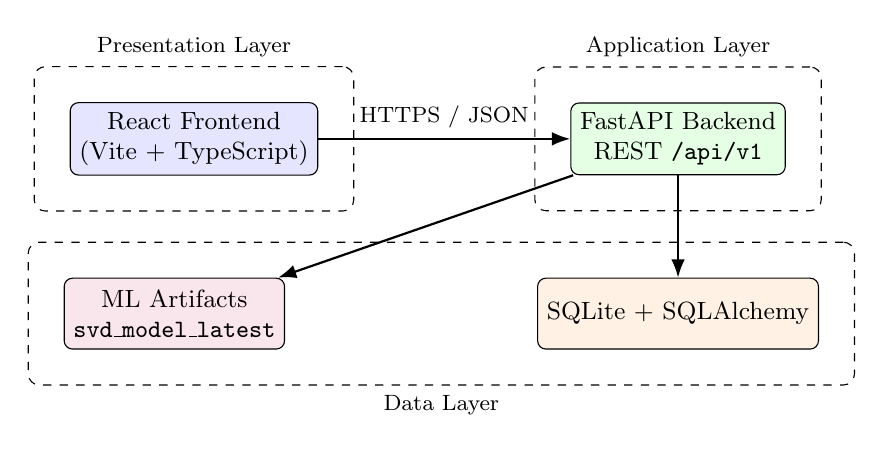
\begin{tikzpicture}[
  >=Latex,
  node distance=1.1cm and 1.4cm,
  every node/.style={font=\small},
  box/.style={draw, rounded corners=3pt, minimum width=2.6cm, minimum height=0.9cm, align=center},
  layer/.style={draw, dashed, inner sep=0.45cm, rounded corners}
]
\node[box, fill=blue!10] (ui) {React Frontend\\(Vite + TypeScript)};
\node[box, fill=green!10, right=3.2cm of ui] (api) {FastAPI Backend\\REST \texttt{/api/v1}};
\node[box, fill=orange!10, below=1.3cm of api] (db) {SQLite + SQLAlchemy};
\node[box, fill=purple!10, left=3.2cm of db] (ml) {ML Artifacts\\\texttt{svd\_model\_latest}};

\draw[->, thick] (ui) -- node[above, font=\footnotesize]{HTTPS / JSON} (api);
\draw[->, thick] (api) -- (db);
\draw[->, thick] (api) -- (ml);

\node[layer, fit=(ui), label={[font=\footnotesize]above:Presentation Layer}] {};
\node[layer, fit=(api), label={[font=\footnotesize]above:Application Layer}] {};
\node[layer, fit=(db) (ml), label={[font=\footnotesize]below:Data Layer}] {};
\end{tikzpicture}
\caption{Three-tier system architecture for the book recommendation system.}
\label{fig:architecture}
\end{figure}

\section{Backend Design}

The backend (\texttt{backend/app/}) is built with \textbf{FastAPI} and \textbf{SQLAlchemy} \cite{fastapi,sqlalchemy}. On startup, tables are created and \texttt{seed\_data()} loads books from \texttt{BX-Books.csv} if the database is empty.

\textbf{API routers:}
\begin{itemize}
    \item \texttt{auth} --- JWT login (\texttt{POST /auth/login})
    \item \texttt{books} --- paginated search, metadata, book detail
    \item \texttt{users} --- profile and preferences
    \item \texttt{recommendations} --- ratings, reading list, personalized recommendations
    \item \texttt{admin} --- book CRUD (admin role only)
    \item \texttt{ml} --- training, metrics, experiments (data scientist only)
    \item \texttt{analytics} --- user activity, popular books, KPIs
    \item \texttt{health} --- service health check
\end{itemize}

\textbf{Role-based access control} uses three roles defined in \texttt{RoleEnum}: \texttt{user}, \texttt{admin}, and \texttt{data\_scientist}. Dependencies (\texttt{require\_role}, \texttt{get\_current\_user}) enforce authorization on protected routes.

\section{Swagger API Documentation Page}

The backend exposes an interactive Swagger UI page for API exploration and manual testing:
\begin{itemize}
    \item Swagger UI: \url{http://127.0.0.1:8000/docs}
    \item OpenAPI JSON: \url{http://127.0.0.1:8000/api/v1/openapi.json}
\end{itemize}

This page documents request/response schemas, authentication requirements, and all available endpoints grouped by tags (\texttt{auth}, \texttt{books}, \texttt{users}, \texttt{recommendations}, \texttt{admin}, \texttt{ml}, and \texttt{analytics}). It is used during development and evaluation to quickly validate endpoint behavior without building custom test clients.

\begin{figure}[htbp]
\centering
\includegraphics[width=0.95\textwidth]{images/swagger.png}
\caption{Swagger UI page showing grouped REST endpoints and authorization requirements for the backend APIs.}
\label{fig:swagger-ui}
\end{figure}

\section{Database Schema}

Core entities include:
\begin{itemize}
    \item \texttt{User} --- credentials, role, genre preferences
    \item \texttt{Book} --- title, author, genre, ISBN, cover, aggregated rating
    \item \texttt{UserRating} --- per-user star ratings (1--5)
    \item \texttt{ReadingListItem} --- planned / reading / completed
    \item \texttt{Recommendation} --- seeded or legacy recommendation rows
    \item \texttt{ModelExperiment}, \texttt{ModelMetrics}, \texttt{ModelJob} --- ML lifecycle
    \item \texttt{AnalyticsUserActivity}, \texttt{AnalyticsPopularBook}, \texttt{AnalyticsTopRatedBook}
\end{itemize}

\section{Frontend Design}

The frontend (\texttt{Bookrecommendationsystemui/}) uses \textbf{React 18}, \textbf{Vite}, \textbf{React Router}, and \textbf{TanStack Query} \cite{react,vite,react_router,tanstack_query}. A shared \texttt{Layout} provides sidebar navigation and a role switcher for demo accounts.

\begin{table}[htbp]
\centering
\caption{Frontend routes and purpose}
\label{tab:routes}
\begin{tabular}{@{}lll@{}}
\toprule
\textbf{Route} & \textbf{Component} & \textbf{Purpose} \\
\midrule
\texttt{/} & Home & Personalized recommendations grid \\
\texttt{/search} & Search & Filtered book search \\
\texttt{/book/:id} & BookDetail & Book metadata and actions \\
\texttt{/profile} & Profile & Reading history and preferences \\
\texttt{/admin} & AdminDashboard & Catalog and analytics (admin) \\
\texttt{/data-scientist} & DataScientistDashboard & ML training and metrics \\
\bottomrule
\end{tabular}
\end{table}

API base URL defaults to \texttt{http://127.0.0.1:8000/api/v1}, configurable via \texttt{VITE\_API\_BASE\_URL}.

\section{Recommendation Serving Flow}
\begin{enumerate}
    \item Client requests \texttt{GET /users/me/recommendations?limit=6} with JWT.
    \item Backend loads \texttt{svd\_model\_latest} from disk.
    \item User ratings are joined to books by \texttt{book\_id} $\rightarrow$ ISBN.
    \item \texttt{estimate\_user\_profile} fits user bias and factors.
    \item Up to 5000 unrated candidate books are scored; top-$N$ returned with reason text.
    \item If SVD path yields no items, seeded recommendations or preference/popularity fallback is used.
\end{enumerate}

\section{Technology Stack}

\begin{table}[htbp]
\centering
\caption{Technology stack}
\label{tab:stack}
\begin{tabular}{@{}ll@{}}
\toprule
\textbf{Layer} & \textbf{Technologies} \\
\midrule
Frontend & React, TypeScript, Vite, Tailwind CSS, shadcn/ui, Recharts \\
Backend & Python 3, FastAPI, SQLAlchemy, Pydantic, python-jose, passlib \cite{fastapi,sqlalchemy,pydantic,jwt_rfc} \\
ML & NumPy, custom SGD matrix factorization \\
Database & SQLite (via SQLAlchemy) \\
Dev tools & pytest, Uvicorn, Alembic \\
\bottomrule
\end{tabular}
\end{table}

\chapter{Dataset Description and Preprocessing}
\chapterdesc{This chapter describes the Book-Crossing dataset used in this project and the preprocessing steps applied for database seeding and model training.}

\section{Book-Crossing Dataset}

The system uses the \textbf{Book-Crossing} dataset \cite{bookcrossing}, a well-known benchmark for recommender systems research. Three CSV files are stored under \texttt{backend/dataset/}:
\begin{itemize}
    \item \texttt{BX-Books.csv} --- ISBN, title, author, year, publisher, cover image URLs
    \item \texttt{BX-Users.csv} --- user demographics (available for extension; not used in current ML pipeline)
    \item \texttt{BX-Book-Ratings.csv} --- User-ID, ISBN, Book-Rating
\end{itemize}

Files use semicolon delimiters and \texttt{latin-1} encoding. Raw explicit ratings are on a 1--10 scale; a value of \textbf{0} indicates implicit feedback (e.g., purchase) and is excluded from training.

Approximate file sizes in this deployment: \texttt{BX-Books.csv} $\sim$75\,MB, \texttt{BX-Book-Ratings.csv} $\sim$30\,MB.

\section{Database Seeding Preprocessing}

Function \texttt{seed\_data()} in \texttt{app/db/seed.py} performs:
\begin{enumerate}
    \item \textbf{Book import} --- Parse \texttt{BX-Books.csv}; deduplicate by ISBN; cap at \texttt{SEED\_BOOK\_LIMIT} (default 20,000).
    \item \textbf{Genre inference} --- Keyword rules on title (e.g., mystery, romance, fantasy) assign a genre label.
    \item \textbf{Rating aggregation} --- Mean explicit rating per ISBN from \texttt{BX-Book-Ratings.csv}, converted to 0--5: $\min(5, \bar{r}/2)$.
    \item \textbf{Demo data} --- Seed users (reader, admin, data scientist), sample recommendations, reading list, and analytics rows.
\end{enumerate}

\section{ML Training Preprocessing}

Function \texttt{load\_ratings\_from\_csv} in \texttt{app/ml/svd.py}:
\begin{enumerate}
    \item Parse ratings; skip invalid rows and implicit zeros.
    \item Scale ratings: $r' = \min(5, r/2)$.
    \item Filter users with fewer than \texttt{min\_user\_ratings} (default 2).
    \item Filter books (ISBN) with fewer than \texttt{min\_book\_ratings} (default 2).
    \item Random subsample to \texttt{max\_ratings} (e.g., 30,000) with fixed \texttt{random\_seed}.
    \item Shuffle and split into train/test by \texttt{test\_ratio} (default 0.2).
\end{enumerate}

\section{Data Quality Considerations}

The Book-Crossing dataset is sparse and noisy: many users rate few books, and ISBNs may not overlap with the seeded application catalog. Inference maps application \texttt{Book.isbn} to model item indices; books outside the training vocabulary are skipped during scoring. Subsampling and filtering improve training stability at the cost of discarding long-tail interactions.

\chapter{AI Pipeline: Training and Deployment}
\chapterdesc{This chapter details the AI pipeline for data training and deployment, from raw ratings CSV through model persistence to live recommendation serving.}

\section{Pipeline Overview}

Figure~\ref{fig:pipeline} summarizes the end-to-end ML workflow from raw CSV to live recommendations.

\begin{figure}[htbp]
\centering
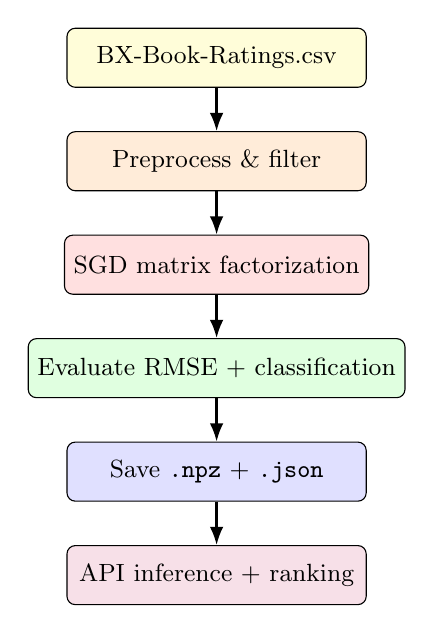
\begin{tikzpicture}[
  >=Latex,
  node distance=0.55cm,
  every node/.style={font=\small},
  pipelinebox/.style={draw, rounded corners=3pt, minimum width=3.8cm, minimum height=0.75cm, align=center}
]
\node[pipelinebox, fill=yellow!15] (csv) {BX-Book-Ratings.csv};
\node[pipelinebox, fill=orange!15, below=of csv] (prep) {Preprocess \& filter};
\node[pipelinebox, fill=red!12, below=of prep] (train) {SGD matrix factorization};
\node[pipelinebox, fill=green!12, below=of train] (eval) {Evaluate RMSE + classification};
\node[pipelinebox, fill=blue!12, below=of eval] (save) {Save \texttt{.npz} + \texttt{.json}};
\node[pipelinebox, fill=purple!12, below=of save] (serve) {API inference + ranking};

\draw[->, thick] (csv) -- (prep);
\draw[->, thick] (prep) -- (train);
\draw[->, thick] (train) -- (eval);
\draw[->, thick] (eval) -- (save);
\draw[->, thick] (save) -- (serve);
\end{tikzpicture}
\caption{AI training and deployment pipeline.}
\label{fig:pipeline}
\end{figure}

\section{Training API}

Data scientists invoke \texttt{POST /api/v1/ml/train} with a JSON body specifying:
\begin{itemize}
    \item Data config: \texttt{max\_ratings}, \texttt{test\_ratio}, \texttt{random\_seed}, \texttt{min\_user\_ratings}, \texttt{min\_book\_ratings}
    \item Base hyperparameters: \texttt{factors}, \texttt{epochs}, \texttt{learning\_rate}, \texttt{regularization}
    \item Optional tuning: \texttt{enable\_tuning}, \texttt{tuning\_space}, \texttt{max\_trials}
\end{itemize}

The handler creates a \texttt{ModelJob}, loads ratings, trains the base configuration, optionally iterates a Cartesian product of tuning parameters (keeping the lowest test RMSE), upserts \texttt{ModelMetrics}, logs \texttt{ModelExperiment} rows, and writes the best model to \texttt{backend/dataset/svd\_model\_latest}.

Minimum 1,000 ratings are required after filtering; otherwise training fails with HTTP 500.

\section{Hyperparameter Tuning}

When \texttt{enable\_tuning} is true, the backend evaluates up to \texttt{max\_trials} combinations from lists such as factors $\in \{50,80,120\}$, epochs $\in \{8,10\}$, learning rates $\in \{0.005,0.01\}$, and regularizations $\in \{0.02,0.05\}$. Each trial is logged as an archived experiment; the best trial by test RMSE is marked active.

\section{Model Artifact Format}

\texttt{save\_model\_artifact} writes:
\begin{itemize}
    \item \texttt{svd\_model\_latest.npz} --- NumPy arrays \texttt{item\_bias}, \texttt{item\_factors}
    \item \texttt{svd\_model\_latest.json} --- \texttt{global\_mean}, \texttt{item\_index} (ISBN $\rightarrow$ index)
\end{itemize}

User factors are \emph{not} persisted; they are recomputed per request from the user's current ratings.

\section{Deployment and Inference}

At runtime, \texttt{recommendations.py} loads the artifact, builds the user profile, scores unrated catalog books, and returns the top-\texttt{limit} items with \texttt{predicted\_rating} rounded to two decimals. Training is synchronous within the HTTP request (suitable for coursework/demo; production would use a background worker).

\section{Seeded Demo Accounts}

\begin{table}[htbp]
\centering
\caption{Demo accounts for testing}
\label{tab:demo-accounts}
\begin{tabular}{@{}ll@{}}
\toprule
\textbf{Email} & \textbf{Role} \\
\midrule
\texttt{alex.johnson@example.com} & user \\
\texttt{admin@example.com} & admin \\
\texttt{datasci@example.com} & data\_scientist \\
\bottomrule
\end{tabular}
\end{table}

Password for all accounts: \texttt{password123}.

\chapter{Evaluation Results}
\chapterdesc{This chapter reports evaluation results with clear metrics, experimental setup, interpretation, and qualitative assessment of recommendation quality.}

\section{Experimental Setup}

Experiments were run using the implementation in \texttt{app/ml/svd.py} with the configuration in Table~\ref{tab:config} (matching the project README quick-start defaults).

\begin{table}[htbp]
\centering
\caption{Training configuration for reported results}
\label{tab:config}
\begin{tabular}{@{}ll@{}}
\toprule
\textbf{Parameter} & \textbf{Value} \\
\midrule
Dataset & \texttt{BX-Book-Ratings.csv} \\
\texttt{max\_ratings} & 30,000 \\
\texttt{test\_ratio} & 0.2 (6,000 test / 24,000 train) \\
\texttt{random\_seed} & 42 \\
\texttt{min\_user\_ratings} / \texttt{min\_book\_ratings} & 2 / 2 \\
\texttt{factors} & 80 \\
\texttt{epochs} & 10 \\
\texttt{learning\_rate} & 0.01 \\
\texttt{regularization} & 0.05 \\
Binary threshold $\tau$ & 3.5 \\
\bottomrule
\end{tabular}
\end{table}

\section{Quantitative Results}

Table~\ref{tab:metrics} reports metrics produced by \texttt{train\_and\_evaluate\_svd} on the held-out test set. Training completed in approximately \textbf{1.53 seconds} for this configuration.

\begin{table}[htbp]
\centering
\caption{Model evaluation metrics (single training run, May 2026)}
\label{tab:metrics}
\begin{tabular}{@{}lr@{}}
\toprule
\textbf{Metric} & \textbf{Value} \\
\midrule
Train RMSE & 0.622 \\
Test RMSE & 0.857 \\
Accuracy (\%) & 77.05 \\
Precision (\%) & 78.31 \\
Recall (\%) & 96.77 \\
F1-score (\%) & 86.57 \\
Training duration (s) & 1.53 \\
Ratings used & 30,000 \\
Distinct users (train index) & 10,688 \\
Distinct books / ISBNs (train index) & 15,674 \\
\bottomrule
\end{tabular}
\end{table}

\section{Interpretation}

\textbf{RMSE:} Test RMSE (0.857) exceeds train RMSE (0.622), indicating mild overfitting---expected with limited epochs and high model capacity relative to noisy data. Values below 1.0 on a 0--5 scale represent reasonable rating prediction for exploratory recommendation.

\textbf{Classification metrics:} High recall (96.8\%) means the model rarely misses books a user would like (at $\tau=3.5$). Precision (78.3\%) is lower, reflecting false positives where the model predicts ``like'' for books the user rated below threshold. F1 (86.6\%) balances these effects. Accuracy (77.1\%) is consistent with class imbalance toward positive labels in the test split.

\textbf{Practical impact:} For the home page, ranking by predicted score prioritizes books likely to receive high stars, supporting discovery even when absolute rating error remains nonzero.

\section{Hyperparameter Sensitivity}

Further trials via \texttt{enable\_tuning} can compare factor counts (50--120), learning rates, and regularization. Lower test RMSE generally correlates with better ranking quality; the data scientist dashboard stores per-trial RMSE in \texttt{ModelExperiment} for comparison.

\section{Qualitative Assessment}

For user \texttt{alex.johnson@example.com} with seeded ratings on three books, the API returns SVD-based recommendations with reason \emph{``Predicted by SVD collaborative filtering from your ratings''} when the artifact exists and ISBNs align. Users without ratings see preference-based or popularity fallbacks, demonstrating graceful degradation.

\chapter{User Interface and Conclusion}
\chapterdesc{This chapter summarizes the user interface surfaces and concludes the report with key achievements and future work directions.}

\section{User Interface Summary}

The Figma-derived UI implements a consistent card-based design (purple accents, rounded corners). Key surfaces include:
\begin{itemize}
    \item \textbf{Home} --- 3-column recommendation grid with cover, rating, genre, and explanation panel.
\end{itemize}

Figure~\ref{fig:ui-home-recommendations} illustrates the Home recommendation interface. The cards display predicted ratings, genres, and explanation text for each recommendation, providing direct evidence that backend recommendation outputs are integrated and rendered in the frontend UI.

\begin{figure}[htbp]
\centering
\includegraphics[width=0.95\textwidth]{images/recommendation_page.png}
\caption{Personalized recommendation interface displaying predicted ratings and recommendation explanations.}
\label{fig:ui-home-recommendations}
\end{figure}

\begin{itemize}
    \item \textbf{Search} --- genre and minimum-rating filters with paginated results.
\end{itemize}

Figure~\ref{fig:ui-search-page} shows the Search interface with query input, genre/rating filters, and paginated book cards for large-catalog exploration.

\begin{figure}[htbp]
\centering
\includegraphics[width=0.95\textwidth]{images/search_book_page.png}
\caption{Search page interface with keyword search, genre/rating filters, and paginated catalog results.}
\label{fig:ui-search-page}
\end{figure}

\begin{itemize}
    \item \textbf{Book Detail} --- metadata, star display, reading-list actions.
    \item \textbf{Profile} --- avatar, preferences, reading history.
    \item \textbf{Admin Dashboard} --- book table with CRUD modals; top-rated chart.
\end{itemize}

Figure~\ref{fig:ui-admin-dashboard} presents the Admin Dashboard analytics area, including the popularity-vs-rating scatter view and per-book rating summaries used to monitor catalog quality.

\begin{figure}[htbp]
\centering
\includegraphics[width=0.95\textwidth]{images/admin_dashboard.png}
\caption{Admin dashboard analytics view showing popularity-versus-rating trends and average rating summaries by book.}
\label{fig:ui-admin-dashboard}
\end{figure}

\begin{itemize}
    \item \textbf{Data Scientist Dashboard} --- model overview, Train/Test RMSE cards, experiment table with activate/remove actions, and training dialog wired to \texttt{POST /ml/train}.
\end{itemize}

Figure~\ref{fig:ui-ds-metrics-versioning} highlights the Data Scientist Dashboard cards for train/test RMSE and model versioning status, while Figure~\ref{fig:ui-ds-experiments} shows the experimentation table used to compare, activate, and remove model runs.

\begin{figure}[htbp]
\centering
\includegraphics[width=0.95\textwidth]{images/evaluation_metrics.png}
\caption{Data Scientist Dashboard cards showing train/test evaluation metrics and production model versioning status.}
\label{fig:ui-ds-metrics-versioning}
\end{figure}

\begin{figure}[htbp]
\centering
\includegraphics[width=0.95\textwidth]{images/model_experimentation.png}
\caption{Model experimentation table with RMSE tracking and actions to set an active model or remove archived experiments.}
\label{fig:ui-ds-experiments}
\end{figure}

\section{Conclusion}

This project delivers an end-to-end book recommendation system with clear stakeholder value: readers receive personalized suggestions, administrators manage catalog data, and data scientists control model training and evaluation. The theoretical foundation rests on collaborative filtering via matrix factorization; the implementation trains efficiently on Book-Crossing data and deploys a compact artifact for real-time inference with online user profiling.

Reported test metrics (RMSE 0.857, F1 86.6\%) demonstrate that the pipeline produces a functional model suitable for demonstration and coursework evaluation.

\section{Future Work}
\begin{itemize}
    \item Persist full user factors or use two-tower retrieval for faster candidate generation.
    \item Incorporate content features (author, genre embeddings) for hybrid recommendations and cold-start books.
    \item Replace synchronous training with job queues (Celery/RQ) and model versioning.
    \item Use production database (PostgreSQL) and containerized deployment.
    \item Conduct A/B tests on click-through and reading-list conversion.
    \item Expand evaluation with ranking metrics (NDCG@K, MAP@K).
\end{itemize}

\clearpage
\appendix
\chapter{API Endpoint Summary}

\begin{table}[htbp]
\centering
\small
\caption{Selected REST API endpoints}
\begin{tabular}{@{}lll@{}}
\toprule
\textbf{Method} & \textbf{Path} & \textbf{Auth} \\
\midrule
POST & \texttt{/auth/login} & Public \\
GET & \texttt{/books} & Public \\
GET & \texttt{/users/me/recommendations} & User \\
PUT & \texttt{/users/me/ratings/\{book\_id\}} & User \\
GET/POST & \texttt{/admin/books} & Admin \\
PATCH/DELETE & \texttt{/admin/books/\{book\_id\}} & Admin \\
POST & \texttt{/ml/train} & Data scientist \\
POST & \texttt{/ml/experiments/\{experiment\_id\}/activate} & Data scientist \\
DELETE & \texttt{/ml/experiments/\{experiment\_id\}} & Data scientist \\
GET & \texttt{/ml/metrics} & Data scientist \\
GET & \texttt{/analytics/user-activity} & Data scientist \\
\bottomrule
\end{tabular}
\end{table}

\chapter{Sample Training Request}

The following command illustrates how a data scientist triggers SVD training via the API (replace \texttt{<TOKEN>} with a valid JWT):

\begin{small}
\begin{verbatim}
curl -X POST "http://127.0.0.1:8000/api/v1/ml/train" \
  -H "Authorization: Bearer <TOKEN>" \
  -H "Content-Type: application/json" \
  -d '{"max_ratings":30000,"test_ratio":0.2,
       "hyperparameters":{"factors":80,"epochs":10,
       "learning_rate":0.01,"regularization":0.05}}'
\end{verbatim}
\end{small}

\chapter{Source Code Layout}

\begin{small}
\begin{verbatim}
figma/
  backend/app/main.py       # FastAPI entry
  backend/app/ml/svd.py     # Training & inference
  backend/app/db/models.py  # SQLAlchemy models
  backend/dataset/          # BX CSV & model artifact
  Bookrecommendationsystemui/src/app/pages/
\end{verbatim}
\end{small}

\clearpage
\phantomsection
\addcontentsline{toc}{chapter}{References}
\begin{thebibliography}{99}

\bibitem{bookcrossing}
Ziegler, C.-N., McNee, S. M., Konstan, J. A., and Lausen, G.:
\newblock Improving Recommendation Lists Through Topic Diversification.
\newblock In \emph{Proceedings of the 14th International Conference on World Wide Web (WWW)}, 2005.
\newblock (Book-Crossing dataset.)

\bibitem{matrix_factorization}
Koren, Y., Bell, R., and Volinsky, C.:
\newblock Matrix Factorization Techniques for Recommender Systems.
\newblock \emph{Computer}, 42(8):30--37, 2009.

\bibitem{recommender_systems_handbook}
Ricci, F., Rokach, L., and Shapira, B. (eds.):
\newblock \emph{Recommender Systems Handbook}.
\newblock Springer, 2015.

\bibitem{ir_book}
Manning, C. D., Raghavan, P., and Sch\"utze, H.:
\newblock \emph{Introduction to Information Retrieval}.
\newblock Cambridge University Press, 2008.

\bibitem{fastapi}
Ramírez, S.:
\newblock FastAPI Documentation.
\newblock \url{https://fastapi.tiangolo.com/}, 2024.

\bibitem{react}
Meta Open Source:
\newblock React Documentation.
\newblock \url{https://react.dev/}, 2024.

\bibitem{vite}
Vite Team:
\newblock Vite Documentation.
\newblock \url{https://vite.dev/guide/}, 2024.

\bibitem{react_router}
React Router Team:
\newblock React Router Documentation.
\newblock \url{https://reactrouter.com/}, 2024.

\bibitem{tanstack_query}
TanStack:
\newblock TanStack Query Documentation.
\newblock \url{https://tanstack.com/query/latest/docs/framework/react/overview}, 2024.

\bibitem{sqlalchemy}
SQLAlchemy Authors:
\newblock SQLAlchemy Documentation.
\newblock \url{https://docs.sqlalchemy.org/}, 2024.

\bibitem{pydantic}
Pydantic Team:
\newblock Pydantic Documentation.
\newblock \url{https://docs.pydantic.dev/}, 2024.

\bibitem{jwt_rfc}
Jones, M., Bradley, J., and Sakimura, N.:
\newblock JSON Web Token (JWT), RFC 7519.
\newblock IETF, 2015.

\bibitem{project_readme}
Book Recommendation Project:
\newblock \texttt{backend/README.md} and \texttt{Bookrecommendationsystemui/README.md}.
\newblock Repository documentation, 2026.

\end{thebibliography}

\end{document}
